% GENERATED by haipipe-display scripts/build_preview.py: page 1 the display, pages 2+ how it was made. Rerun it.
\documentclass[12pt]{article}
\usepackage[letterpaper,margin=1in]{geometry}
\usepackage{fontspec}
\IfFontExistsTF{TeX Gyre Termes}{\setmainfont{TeX Gyre Termes}}{\IfFontExistsTF{Times New Roman}{\setmainfont{Times New Roman}}{}}
\usepackage{microtype}
\usepackage{graphicx,booktabs,tabularx,multirow,array,longtable,amsmath,amssymb,setspace,caption,float,xcolor}
\usepackage{fancyhdr}
\onehalfspacing
\setlength{\parindent}{0.25in}
\setlength{\parskip}{0.35em}
\pagestyle{fancy}\fancyhf{}
\renewcommand{\headrulewidth}{0pt}
\fancyfoot[C]{\thepage}
\usepackage{float}
\begin{document}
\makeatletter\renewcommand{\fps@figure}{H}\renewcommand{\fps@table}{H}\makeatother
\renewcommand{\figurename}{Figure}\renewcommand{\tablename}{Table}\renewcommand{\thefigure}{1}\renewcommand{\thetable}{1}
\begin{figure}
  \centering
  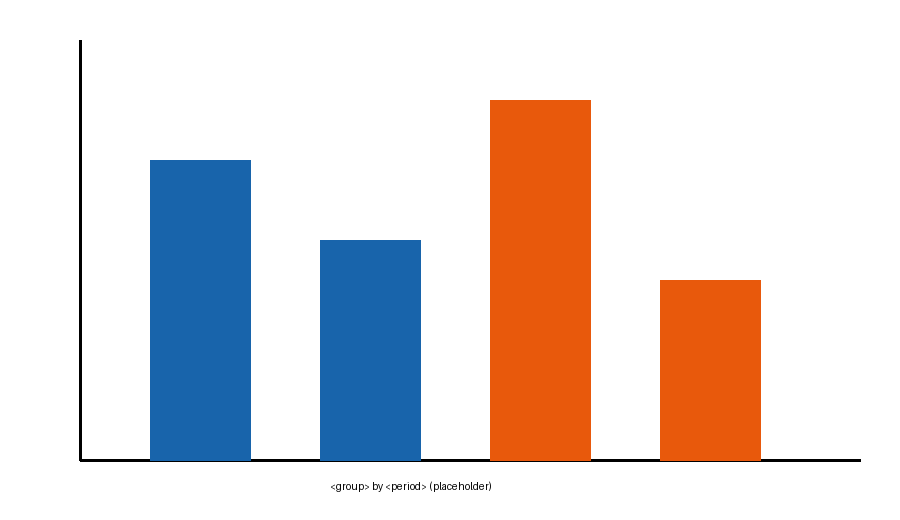
\includegraphics[width=\linewidth]{assets/figure.png}
  \caption{\textbf{<Outcome> by <group>, before and after <the policy>.} Bars show the mean <outcome> per <unit>. Placeholder figure of Tools' Paper-Example; no real data.}
  \label{fig:example}
\end{figure}

\clearpage
\section*{How this display was made}
\subsection*{Data}
<The data source>, years <YYYY to YYYY>.

\subsection*{Sample}
\begin{itemize}\item <who is in it>
\item <how they were chosen>
\end{itemize}
\subsection*{Method}
<The comparison or model, and its estimator.>

\subsection*{Outcomes}
\begin{enumerate}\item \textbf{<outcome>}: <its definition>
\end{enumerate}
\subsection*{Made by}
\begin{itemize}\item \texttt{work/b01\_<block>/j01\_<job>/t01\_<task>/runs/r01\_<run>/result/}
\end{itemize}
\subsection*{Numbers}
Read from the Result files above; none is a screen reading.

\end{document}
